\section{Conditions and geometries}
\label{sec:condgeom}
\label{sec:geom}

\textbf{Purpose.} This section fixes the three states every number in this report is read at, and
says what was changed on the wing. Five candidates are compared against one rigid baseline. Each
moves a different part of the outer wing by a different amount. Every geometric number here is
read from the design files and the delivered section schedules, and mesh statistics are quoted
where they bear on the geometry.
\subsection{Operating points}
\label{sec:cond}
\label{sec:cond:points}

\textbf{Purpose.} Three states are fixed here, and every number in this report is read at one of
them. Two are cruise states of the ARGUS aircraft at $M = 0.78$. One is the low-speed point the DSO
optimisation selected its candidates at. Table~\ref{tab:cond:points} is the record of what ran.
\textbf{``Condition~CR'' is the low-speed point, and CR does not stand for cruise.} It is the
$M = 0.10$ state the design study selected its candidates at, and it is named Condition~CR
throughout this report and in the delivered packages. The two states that \emph{are} cruise are
always written ``early cruise'' and ``late cruise'', both at $M = 0.78$. The distinction is
load-bearing and the wrong reading inverts results: where Section~\ref{sec:hinge} reports a
penalty that is smaller at Condition~CR than at early cruise, reading CR as cruise makes the
sentence contradict itself. Wherever this report says ``cruise'' without qualification it means
the two $M = 0.78$ states and never Condition~CR.

\textbf{Method.} Each cruise state is pinned by mass, altitude and Mach number. Standard-atmosphere
density and speed of sound follow from the altitude. The target lift coefficient is then
$C_{L,\mathrm{target}} = W / (q_\infty S_\mathrm{ref})$. Every value in
Table~\ref{tab:cond:points} is read from the recipes' \texttt{CONDITION.json} and from each built
case's own \texttt{forceCoeffs} block.

\textbf{Scale.} The cruise states are defined at aircraft scale, on a chord of $3.196$~m. The
meshed geometry is model scale, on $C_\mathrm{ref} = \num{0.393957}$~m. Viscosity is set so that
Reynolds number on the model chord equals the aircraft-scale value. The table therefore carries a
model-scale $\mu$ beside an aircraft Reynolds number.

\begin{table}[htbp]
  \centering
  \footnotesize
  \caption{The three operating points. Coefficients are on the DSO basis,
  $S_\mathrm{ref} = \num{1.24092}$~m$^2$ and $C_\mathrm{ref} = \num{0.39396}$~m; the RANS cases
  solve a half wing at $A_\mathrm{ref} = \num{0.620462}$~m$^2$. Reynolds number is on the DSO
  chord: at Condition~CR it is $0.79$ million on the TP-1580 chord of $\num{0.3404}$~m, which is
  the figure in wider circulation. Condition~CR is solved incompressible, so its pressure is
  kinematic and its temperature is not defined; the tabulated $q_\infty$ is
  $\tfrac{1}{2}\rho_\infty|U_\infty|^2$ on the $\rho_\infty = 1.225$ its \texttt{forceCoeffs}
  block carries. Our cruise $q_\infty$ runs $0.303$~per~cent above Zheng's
  Table~18~\cite{zheng} at both states, common mode within our runs.}
  \label{tab:cond:points}
  \begin{tabular}{lrrr}
    \toprule
                                        & Condition CR      & Early cruise            & Late cruise \\
    \midrule
    Case prefix                         & \texttt{SW*}      & \texttt{CMP*}           & \texttt{LC*} \\
    Flight state                        & DSO-matched       & \num{74500}~kg, 10~km   & \num{56000}~kg, 12~km \\
    Mach                                & $0.10$            & $0.78$                  & $0.78$ \\
    Target $C_L$                        & $0.428277635108$  & $0.529297087450$        & $0.544114800210$ \\
    $|U_\infty|$ (m/s)                  & $34.0$            & $233.934028$            & $230.501789$ \\
    $\rho_\infty$ (kg/m$^3$)            & $1.225$           & $0.41271$               & $0.31083$ \\
    $T_\infty$ (K)                      & n/a               & $223.15$                & $216.65$ \\
    $p_\infty$ (Pa)                     & n/a (gauge)       & $\num{26495.90}$        & $\num{19373.96}$ \\
    $q_\infty$ (Pa)                     & $708.05$          & $\num{11292.80}$        & $\num{8257.37}$ \\
    Viscosity                           & $\nu\,1.46\times10^{-5}$ & $\mu\,1.7961143\times10^{-6}$ & $\mu\,1.7523444\times10^{-6}$ \\
    $Re_{C_\mathrm{ref}}$               & $0.92\times10^{6}$ & $2.1176454\times10^{7}$ & $1.6107442\times10^{7}$ \\
    Solver                              & incompressible    & compressible            & compressible \\
    Turbulence model                    & kOmegaSST         & Spalart--Allmaras       & Spalart--Allmaras \\
    Wall treatment                      & resolved          & modelled                & modelled \\
    \bottomrule
  \end{tabular}
\end{table}
\textbf{Why the two cruise states differ.} The aircraft burns fuel and steps from 10 to 12~km, so
mass falls by a quarter and density falls with the altitude. Dynamic pressure falls faster than
weight, so the required lift coefficient rises by $2.80$~per~cent while Reynolds number drops by
$24$~per~cent.

\textbf{The two states close against each other.} At fixed reference area the ratio of targets
equals the mass ratio over the dynamic-pressure ratio. The targets give $1.0279951$. Mass and
dynamic pressure give $1.0279974$, agreeing to $2.3\times10^{-6}$ relative. The two points are one
flight state read at two masses.

\subsection{The wing every candidate starts from}
\label{sec:geom:baseline}

\textbf{Baseline.} All six surfaces are the same NASA EET AR-12 cruise wing. Only the outer wing
differs between them. Fuselage, tail and high-lift system are not modelled.
Table~\ref{tab:geom:planform} gives the planform an experimentalist would need.

\textbf{Section.} The aerofoil is a supercritical section of $11.97$~per~cent thickness. Its
trailing edge is blunt at $0.63$~per~cent of local chord. That edge is $1.03$~mm at the tip and
sets the surface cell size everywhere.

\begin{table}[htbp]
  \centering
  \footnotesize
  \caption{Baseline planform, read from the geometry sidecar of the surface the cases mesh,
  \texttt{geometry/derived/wing3d/baseline\_oml\_placed.json}. Measured values are taken from the
  lofted surface; targets are the registered references. The half-wing planform area integrates
  to \num{0.620463}~m$^2$ against the $A_\mathrm{ref} = \num{0.620462}$~m$^2$ the cases carry.
  The meshing surface adds a $20$~mm root extension through the symmetry plane as scaffolding,
  which is cut away and is not part of the wing.}
  \label{tab:geom:planform}
  \begin{tabular}{lrrl}
    \toprule
    Quantity & Measured & Target & Note \\
    \midrule
    Root chord (m)                  & $0.639125$  & $0.640081$ & \\
    Tip chord (m)                   & $0.152172$  & $0.152400$ & taper ratio $0.238$ \\
    Semispan (m)                    & \multicolumn{2}{r}{$b_\mathrm{ref}/2 = 1.8288$} & half model on a symmetry plane \\
    Leading-edge sweep (deg)        & $28.8447$   & $28.8620$  & quarter chord $27$ \\
    Tip minus root twist (deg)      & $-4.129406$ & $-4.11495$ & washout \\
    Root incidence (deg)            & $1.852649$  & $1.873$    & placement transform \\
    Dihedral rise over semispan (m) & $0.130498$  & $0.139$    & placement transform \\
    Half planform area (m$^2$)      & \multicolumn{2}{r}{$0.620463$} & integrated from the section table \\
    Thickness, trailing edge        & \multicolumn{2}{r}{$11.97\,\%$ chord; TE $0.63\,\%$ local chord} & TE $1.03$~mm minimum \\
    \bottomrule
  \end{tabular}
\end{table}

\textbf{Span coordinate.} Stations below are quoted in $\eta = y/(b/2)$. The wing is lofted
through 19 defining stations. Those stations carry the morphing, and every realised value in this
section is read at them.

\subsection{Two lineages of the same wing}
\label{sec:geom:lineage}

\textbf{Why there are two.} The delivered design file lofts the wing through 19 stations but
carries only 9 distinct aerofoils: ten stations inherit a neighbour's section instead of a
blended one, so thickness is held constant across runs of stations and then steps. A corrected
file was issued afterwards in which all 19 stations carry their own aerofoil. The meshed
baseline is the uncorrected file. All five candidates are built on the corrected one.

\textbf{What the difference is.} Figure~\ref{fig:geom:lineage} shows it. Both wings are the
same planform at the same twist, so the difference is thickness and nothing else. They agree
exactly at every station both files define and differ only between those stations, which is
why the uncorrected thickness distribution is a staircase and the corrected one a smooth
taper. The difference is zero at and inboard of $\eta = 0.450$. The first station that differs,
$\eta = 0.515$, is also the largest, at $0.407$ percentage points of $t/c$ and $0.209$~per~cent
of chord in surface ordinate. Camber differs by at most $0.0034$~per~cent of chord, two orders
of magnitude below the thickness difference.

\textbf{What it costs the comparison.} Nothing for the candidate ranking. All five candidates
share the corrected lineage, so the difference is common to both sides of every
candidate-to-candidate number in this report and cancels from it. It enters only where a
candidate is differenced against the meshed baseline, and there it is bounded by the figures
above.

\begin{figure}[htbp]
  \centering
  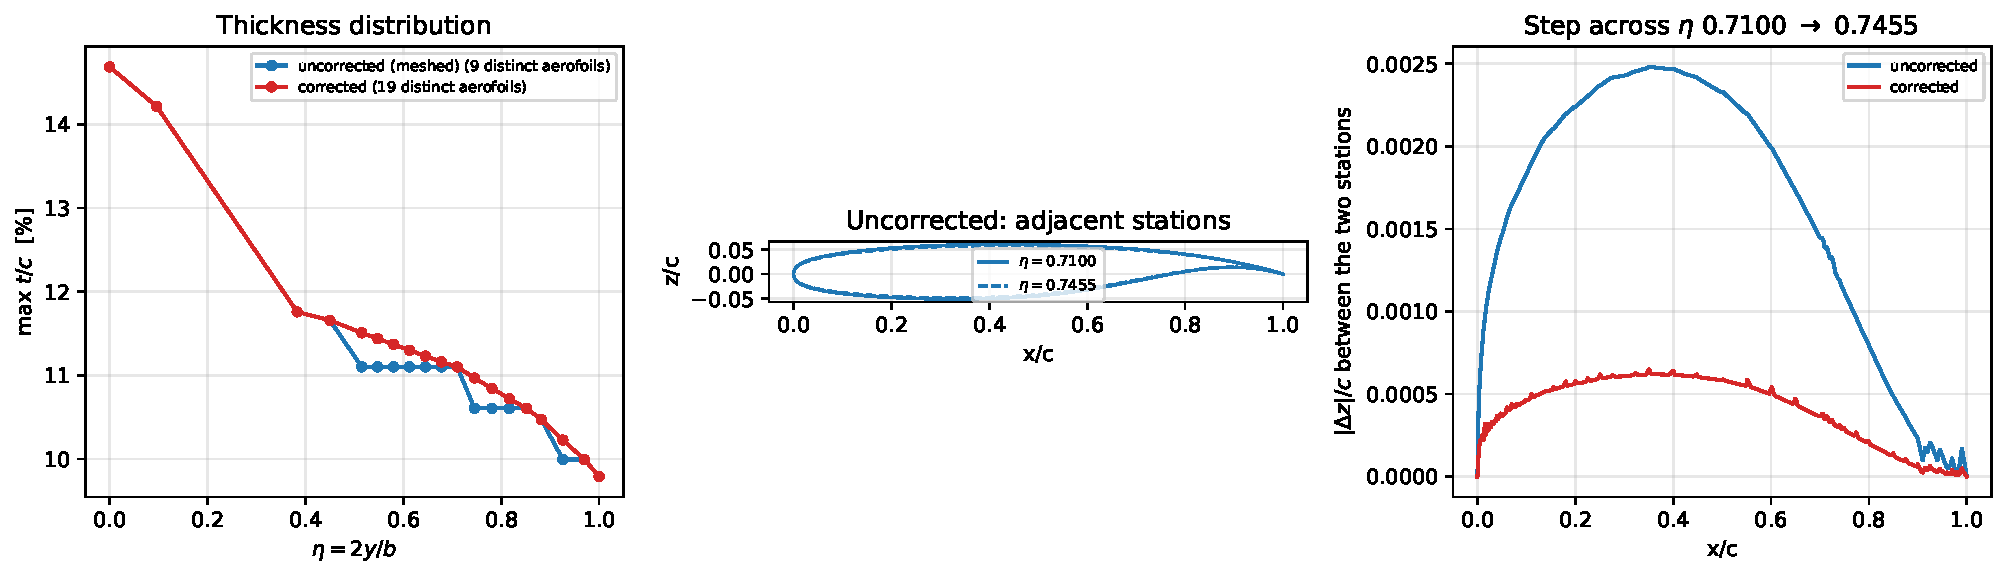
\includegraphics[width=0.94\linewidth]{fig/fig_lineage_staircase.pdf}
  \caption{The two lineages of the baseline wing. Left: maximum $t/c$ against $\eta$, the
  uncorrected file (9 distinct aerofoils across 19 stations) against the corrected file (19).
  The uncorrected curve holds thickness constant across runs of stations and steps between
  them; the corrected curve tapers. Centre: the two adjacent uncorrected stations either side
  of the largest step, overlaid, which is what an inherited rather than blended section looks
  like. Right: the surface ordinate difference $|\Delta z|/c$ across that step for each
  lineage; the uncorrected step reaches $0.25$~per~cent of chord where the corrected reaches
  $0.06$. Measured from the two design files by
  \texttt{scripts/measure\_lineage\_pair.py} into \texttt{data/lineage\_measured.json}.}
  \label{fig:geom:lineage}
\end{figure}

\subsection{How the morphing is commanded}
\label{sec:geom:law}

Three mechanisms appear across the five candidates. Each acts on a different part of the section.

\textbf{Continuous trailing-edge camber (C, F, M).} Camber changes behind a fixed start line at
$x_h/c = 0.62$. Let
\begin{equation}
  \xi = \frac{x/c - x_h/c}{1 - x_h/c}, \qquad 0 \le \xi \le 1 .
\end{equation}
The camber displacement follows a smoothstep in $\xi$,
\begin{equation}
  S(\xi) = 3\xi^{2} - 2\xi^{3}, \qquad
  \Delta z_c(x,\eta) = -A(\eta)\,S(\xi), \qquad x/c \ge x_h/c .
\end{equation}
Both $S$ and its slope vanish at the start line. The moving surface therefore leaves the fixed
forward aerofoil without a step or a slope break. Upper and lower surfaces are displaced by the
same increment, so thickness is preserved by construction. The delivered sections carry zero
change in $t/c$ and a trailing-edge displacement equal to $-A/c$ to $10^{-9}$. Positive $A$ is
trailing edge down. The amplitude $A/c$ is normalised on the \emph{local} chord.

\textbf{Distributed twist (W).} The whole local section rotates about $x/c = 0.25$. The aerofoil
profile is unchanged and only incidence moves. The command is an incremental twist in degrees,
added to the baseline washout. This is the one candidate whose leading edge moves.

\textbf{Conventional hinged (H).} Two aileron-like segments rotate rigidly about a hinge at
$x_h/c = 0.70$. Deflection is constant within a segment and steps between them. The slope breaks
at the hinge, which is what separates this concept from camber morphing. It is modelled as a
zero-gap outer mould line, with no gap, seal or bracket represented.

\textbf{Command layout.} Each continuous concept carries five spanwise commands. These are design
variables and not geometric sections. Values between them are interpolated onto the 19 defining
stations before the surface is lofted. Table~\ref{tab:geom:command} gives the commands as the
design files hold them.

\begin{table}[htbp]
  \centering
  \scriptsize
  \setlength{\tabcolsep}{4pt}
  \caption{The six geometries and the command each flies, read from the DSO design files
  (\texttt{<case>\_design.json}) and \texttt{registry/candidates.yaml}. Camber commands are $A/c$
  on the local chord at $\eta = 0.60$, $0.70$, $0.80$, $0.90$, $1.00$. Twist commands are
  $\Delta\theta$ in degrees at $\eta = 0.68$, $0.76$, $0.84$, $0.92$, $1.00$, positive leading
  edge up. The hinged command is the inboard and outboard segment deflection in degrees, positive
  trailing edge down. The STL column is the SHA-256 prefix of the placed surface the cases mesh.
  All five candidates were selected at Condition~CR, $M = 0.10$, $C_L = 0.428277635108$
  (Table~\ref{tab:cond:points}).}
  \label{tab:geom:command}
  \begin{tabular}{lllll}
    \toprule
    ID & DSO case & Concept & Command & STL \\
    \midrule
    B & \texttt{baseline\_wing\_only\_refined} & rigid     & none & \texttt{20bd6acd} \\
    C & \texttt{cte\_i002\_c04}  & TE camber & $0.016427$, $0.021826$, $0.033726$, $0.015955$, $0.000015$ & \texttt{790c3ded} \\
    F & \texttt{cfft\_b02\_c01}  & TE camber & $0.012607$, $0.013869$, $0.012069$, $0.012284$, $0.000461$ & \texttt{82bf2e1e} \\
    M & \texttt{mcv2\_i002\_c01} & TE camber & $0.008027$, $0.025978$, $0.034968$, $0.018199$, $0.000218$ & \texttt{dae22d0c} \\
    W & \texttt{cffw\_b01\_c01}  & twist     & $+1.7997$, $+1.1260$, $+1.2782$, $+0.2573$, $-0.9994$ & \texttt{200fa64c} \\
    H & \texttt{chc\_g02\_c06}   & hinged    & $2.4954$ inboard, $1.6636$ outboard & \texttt{18329aa3} \\
    \bottomrule
  \end{tabular}
\end{table}

\textbf{Two generations, not five designs.} C and M come from the July selection. F, W and H come
from the August reselection, after the design study moved from near-field to far-field induced
drag. C and F are the same concept ranked under two metrics. F's peak amplitude is $41$~per~cent
of C's.

\subsection{What each candidate actually moves}
\label{sec:geom:delta}

\textbf{Method.} Commands are interpolated onto the defining stations, so the realised peak sits
at a station rather than at a control point. The chord tapers by a factor of $4.2$ from root to
tip. A constant $A/c$ therefore produces a falling physical displacement outboard.
Table~\ref{tab:geom:delta} gives commanded amplitude and realised displacement together, and
Figure~\ref{fig:geom:displacement} shows the same thing on the wing.

\begin{figure}[htbp]
  \centering
  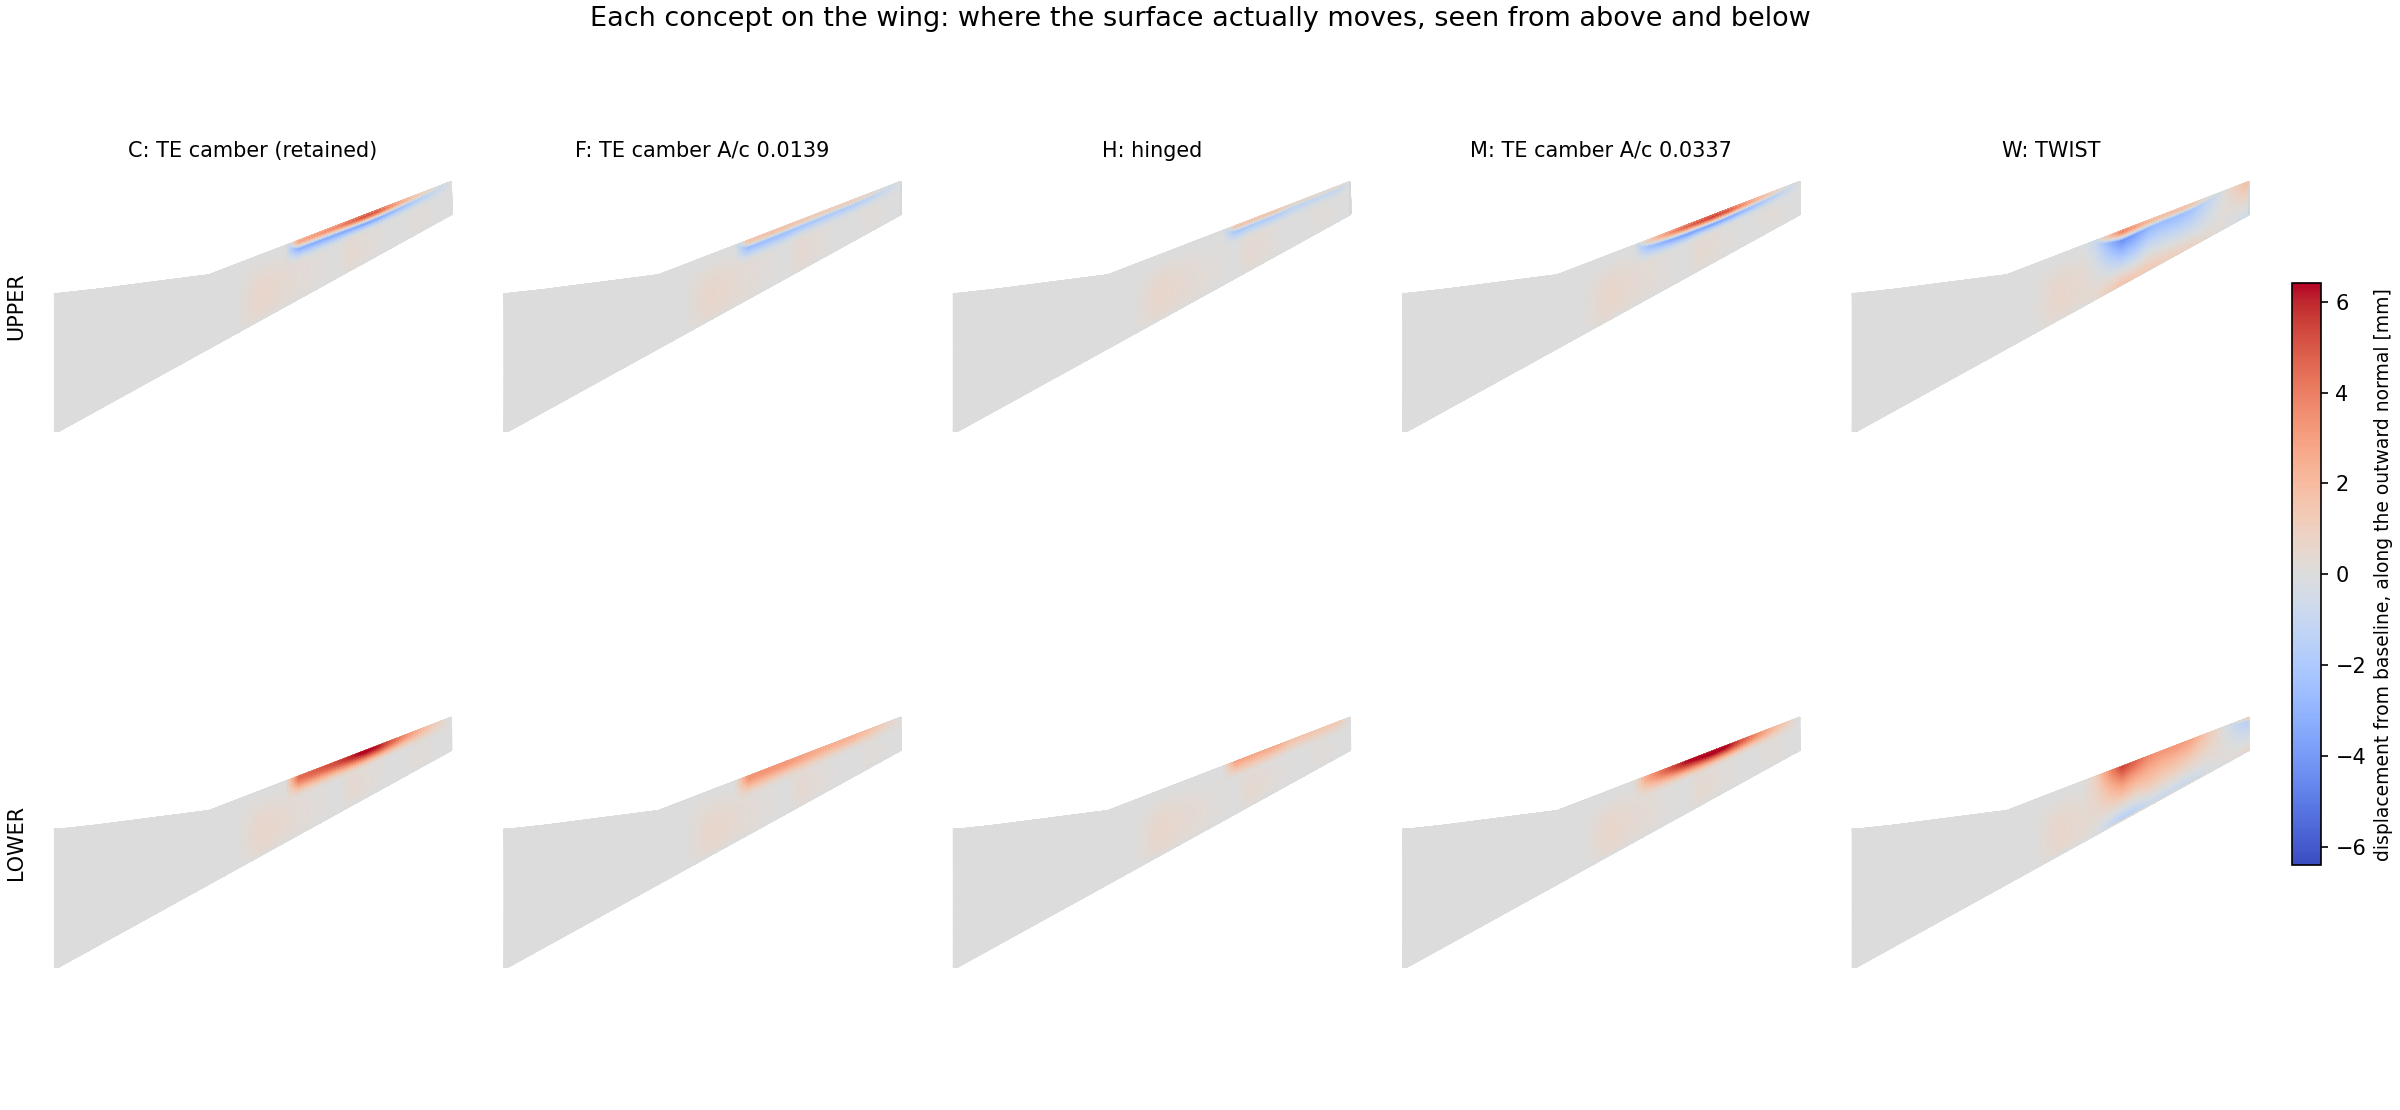
\includegraphics[width=\linewidth]{fig/concept_displacement_3d.png}
  \caption{Where each concept moves the surface, seen from above and below. Panel letters are the
  geometry IDs of Table~\ref{tab:geom:command}. Span runs left to right with the root at left and
  chord up the page. Colour is displacement from the baseline surface measured along the
  baseline's own outward normal, so the same colour means the same physical direction on both
  surfaces: the four camber concepts move the lower surface down and the upper surface up over
  the aft wing, and W, a rigid rotation about $x/c = 0.25$, moves the whole section including the
  leading edge, which is the signature that distinguishes a twist from a camber morph. One
  colour scale spans every panel, $\pm 6.42$~mm at the $99.5$th percentile, because per-panel
  autoscaling would make five different magnitudes look alike. Surfaces are matched by nearest
  point rather than by vertex index, since the three later concepts carry \num{195266} triangles
  against the baseline's \num{192588}. Generated by \texttt{scripts/render\_concept\_3d.py}.}
  \label{fig:geom:displacement}
\end{figure}

\begin{table}[htbp]
  \centering
  \footnotesize
  \setlength{\tabcolsep}{4pt}
  \caption{Realised geometry change at the 19 defining stations. Computed from the delivered
  schedules: \texttt{<case>\_section\_schedule.csv} for C, F, M and H, and
  \texttt{cffw\_b01\_c01\_twist\_schedule.csv} for W. ``Peak command'' is the largest amplitude
  reached at a defining station. It is $A/c$ for the camber candidates and degrees for W and H.
  ``Peak TE'' is the largest trailing-edge displacement in millimetres, with the station it
  occurs at. For W the trailing edge travels on an arc, and the entry is
  $0.75\,c\sin\Delta\theta$ derived from the tabulated twist and chord. Displacement is trailing
  edge down in every case except W outboard of $\eta = 0.95$.}
  \label{tab:geom:delta}
  \begin{tabular}{llrrrrr}
    \toprule
    ID & Acts over & Stations & Peak command & at $\eta$ & Peak TE (mm) & at $\eta$ \\
    \midrule
    C & $\eta$ $0.6125$ to tip & 12 & $0.031465$   & $0.781$ & $6.894$ & $0.781$ \\
    F & $\eta$ $0.6125$ to tip & 12 & $0.013689$   & $0.710$ & $3.452$ & $0.6125$ \\
    M & $\eta$ $0.6125$ to tip & 12 & $0.033260$   & $0.781$ & $7.288$ & $0.781$ \\
    W & $\eta$ $0.6125$ to tip & 12 & $+1.7435$~deg & $0.6775$ & $5.719$ & $0.6775$ \\
    H & $\eta$ $0.710$ to $0.970$ & 8 & $2.4954$~deg & $0.710$ & $3.145$ & $0.710$ \\
    \bottomrule
  \end{tabular}
\end{table}

\textbf{Result.} Every candidate moves the wing by millimetres. The largest movement anywhere in
the set is $7.29$~mm, on M. That is $1.1$~per~cent of the root chord. C follows at $6.89$~mm and
W at $5.72$~mm. F and H are the smallest at $3.45$ and $3.15$~mm.

\textbf{Taper moves the peak.} F shows the effect plainly. Its command peaks at $\eta = 0.710$,
but its physical displacement peaks at $\eta = 0.6125$, the innermost morphed station. The chord
there is $0.270$~m against $0.241$~m. C and M peak in both measures at the same station, because
their commands rise steeply enough to beat the taper.

\textbf{The tip is where the concepts part.} All three camber candidates close to near zero at the
tip: $0.002$~mm on C, $0.033$~mm on M and $0.070$~mm on F. W does the opposite. It reaches
$+1.74$~deg of washin at $\eta = 0.6775$, crosses zero between $\eta = 0.926$ and $0.970$, and
ends at $-0.999$~deg of washout at the tip. W is the only bidirectional candidate in the set, and
the only one that unloads the tip by rotating it.

\textbf{H is discrete where the others are smooth.} Its inboard segment holds $2.4954$~deg from
$\eta = 0.710$ to $0.852$. Its outboard segment holds $1.6636$~deg to $\eta = 0.970$. Deflection
steps by $0.832$~deg at the segment break. The outer $3$~per~cent of span carries no deflection
at all.

\subsection{Where the morphing acts in span}
\label{sec:geom:span}

\textbf{Region.} The continuous concepts act over $\eta = 0.60$ to the tip. That interval is
$25.2$~per~cent of the half-wing planform, taper making it far less than the $40$~per~cent of
span it occupies. Only the chord aft of $x_h/c = 0.62$ moves, so the moving surface is
$9.6$~per~cent of the half-wing planform. H acts over $\eta = 0.710$ to $0.970$, which is
$15.4$~per~cent of planform, and moves $4.6$~per~cent aft of its hinge.

\textbf{Measured effect.} Where that geometry appears in the loading is shown in
Section~\ref{sec:cr:loads}, Figure~\ref{fig:geom:spanwise}: the difference from baseline sits over
the morphed span in every case.

\subsection{Meshed surfaces and their statistics}
\label{sec:geom:mesh}

\textbf{Route.} All six surfaces are lofted by one procedure, step for step, but that procedure
was run twice: B, C and M went through it in July and F, W and H in August, and the two runs
differ only in the tip-cap construction. Each is tessellated at
200 chordwise points per surface and 240 spanwise stations, with the 19 defining stations
retained. The same placement transform and the same blunt-trailing-edge convention follow.
Table~\ref{tab:geom:mesh} gives the surfaces and the meshes built on them.

\begin{table}[htbp]
  \centering
  \footnotesize
  \setlength{\tabcolsep}{5pt}
  \caption{Meshed surfaces and as-built mesh size, on the meshes every result in this report is
  taken from. Triangle counts are from each surface's own sidecar and split by delivery, not by concept.
  Condition~CR counts are the \texttt{checkMesh} figures carried by the run cards; cruise counts
  are from each mesh's own \texttt{polyMesh/owner} header. The surface gate is
  \texttt{surfaceCheck} on the case copy: zero open edges, zero over-connected edges, one zone
  and one normal orientation. Mesh recipe and layer stacks are in Section~\ref{sec:setup:mesh}. Source: rows generated by
  \texttt{scripts/make\_cruise\_tables.py}.}
  \label{tab:geom:mesh}
  \begin{tabular}{lllrrrl}
    \toprule
    ID & Concept & Triangles & Cells, Condition CR & Cells, early cruise & Cells, late cruise & Surface gate \\
    \midrule
\inputrows{sections/gen/tab_geom_mesh_rows.tex}
    \bottomrule
  \end{tabular}
\end{table}

\textbf{What the mesh size tracks.} Nothing but the condition: the six Condition~CR meshes lie
within $0.10$~per~cent of one another and the twelve cruise meshes within $0.15$~per~cent, so
every candidate-minus-baseline difference is taken between meshes of the same size.

\textbf{The integrated surface.} The wing patch carries \num{5276562} to \num{5277100} faces
across the eighteen trim cases, a spread of about one face in $10^{4}$. The surface discretisation is
therefore common to both sides of every candidate-minus-baseline difference. The meshing surface
also carries the $20$~mm root extension, so its STL area of $1.3497$~m$^2$ stands $5.49$~per~cent
above the wing's wetted area of $1.2794$~m$^2$. Wetted area is taken from the solver wing patch.

\subsection{What was changed, in one place}
\label{sec:geom:summary}

\textbf{Decision.} The five candidates are three concepts and two selection generations. They act
on the outer $40$~per~cent of span and move between $3.1$ and $7.3$~mm of trailing edge. C, F and
M differ in amplitude and spanwise placement rather than in mechanism, and all three close to
zero at the tip. W and H are the structurally distinct pair: W rotates whole sections
bidirectionally and is the only candidate that moves a leading edge, and H breaks the surface
slope at a hinge.
